%************************************************
\chapter{Method validation and performance analysis on simulated data}\label{ch:simulations} 
%************************************************
\todo{Complete all the stuff that is missing. Separate the initiailization and method comparison analysis. Rewrite because this is copy paste from paper, check the references, try to fit figures in the text}
\section{Simulating data with a spatial component }
Simulating data with a spatial component is a non-trivial problem. Existing methods rely on MCMC approaches as described in \cite{Chalmond89}. However, in this case with a relatively large number of nodes in the graph ($\sim 34,000$), this is computationally expensive. To overcome this problem, I exploited the fact that the {\it{Platynereis}} dataset already possesses a spatial component. As outlined in Figure \ref{fig:simulationScheme}, the simulation starts by clustering the gene expression data using different values of $K$ and by storing the resulting parameter estimates with the HRMF method described in chapter \ref{ch:HMRF}. Subsequently, I use the values of the estimated parameter $\boldsymbol{\Theta}$ to simulate binarised gene expression data from $K$ clusters where, for cluster $h$, the expression of gene $m$ is simulated from a Bernoulli distribution with parameter $\theta_{m,h}$ as described in \ref{subsec:simul_non_spatial}. This non spatial simulated data is then reintroduced in the spatial context of the biological data \ref{subsec:simul_spatial} leading to a simulated dataset with all parameters being fully determined. In the next paragraphs, I will describe each step of this simulation scheme.

	\begin{figure}[h]
\centerline{\includegraphics[width=\linewidth]{gfx/chapter5/simulation_scheme.png}}
\caption{{\bf Simulation scheme used to generate gene expression data with a spatial component and known parameters.} The values of $\Theta$ are used to generate a dataset of clusters with the same gene expression profile as the reference. Each simulated cell is then assigned to its corresponding spatial localization so that the simulated data keeps the spatial compenent of the biological data.}
\label{fig:simulationScheme}
	\end{figure}
	
	\subsection{Simulating non spatial gene expression data}\label{subsec:simul_non_spatial}
	\subsection{Introducing a known spatial context}\label{subsec:simul_spatial}
	We assign each simulated ``cube" the same spatial location as the corresponding ``cube" in the biological dataset, meaning that both the simulated and the biological datasets have the same neighbouring graph. We can then cluster these simulated datasets using the method outlined above and determine how accurately we can estimate the parameters ($\mathbf{\beta}, \mathbf{\Theta}$) and choose the correct number of clusters, $K$.\\ 
	\subsection{Expected results}\label{subsec:expected_simul_results}

\section{Aligning clustering results }
	\subsection{Theoretical problem in comparing clustering results}
	\subsection{Alignment via similarity-specificity matric}

\section{Validation of parameters estimation and model choosing}

	\subsection{Estimation of beta}
	As well as directly comparing the clusters, we can also determine how accurately the $\mathbf{\beta}$ parameters are estimated. To this end, in Figure \ref{fig:beta_validation} we compare the true and inferred mean values of $\mathbf{\beta}$ for different values of $K$. The values of $\mathbf{\beta}$ increase with $K$, which is to be expected since more clusters implies the existence of more transition areas, thus making an increase of $\mathbf{\beta}$ necessary to maintain the optimal spatial coherency of the model. Figure \ref{fig:beta_validation} also shows a slight but consistent underestimation of $\mathbf{\beta}$. This can be explained by noting that the simulation scheme used may reduce the spatial coherency within clusters. Specifically, as illustrated in Figure \ref{fig:beta_error}, clusters may not display homogeneous expression of a given gene: instead, depending upon the value of $\theta$, a gene will be expressed only in a fraction of cells. In reality, the cells in which such genes are expressed may have a coherent spatial structure within the cluster that is lost in the simulation, thus explaining the consistently smaller value for $\mathbf{\beta}$ that are estimated. To confirm this, we performed a second simulation using the parameter values estimated from the first simulation as a reference. In this context we did not expect any further loss of spatial coherency, which was indeed confirmed as shown by the blue curve in Figure \ref{fig:beta_validation}.\\
	
	\begin{figure}[h]
\centerline{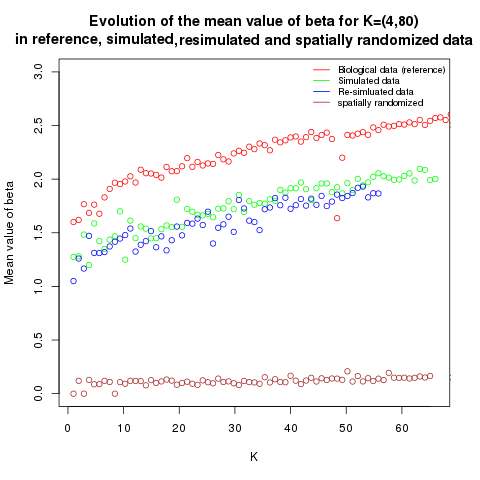
\includegraphics[width=\linewidth]{gfx/chapter5/beta_valid.png}}
\caption{{\bf Validating the estimation of beta.} This figure shows the evolution for $K \in [4,80]$ of the mean value of $\beta$ across all the clusters. The red dots represent the biological data clustering (i.e the reference in our simulations scheme). The green dots represent the results obtained after clustering simulated data, which shows an underestimation of $\beta$. To confirm that this underestimation come from the simulation scheme and not the clustering method, we used the simulated data as the reference to generate a ``second generation" of simulated data, suppressing the simulation scheme bias (see Figure \ref{fig:beta_error}). The results of this re-simulation are shown by the blue dots, which exhibit no underestimation of $\beta$. Finally the brown dots represent the mean value of $\beta$ on the same simulated data but spatially randomized, as expected the $\beta$ are now estimated to $0$.}
\label{fig:beta_validation}
	\end{figure}
	
	\begin{figure}[h]
\centerline{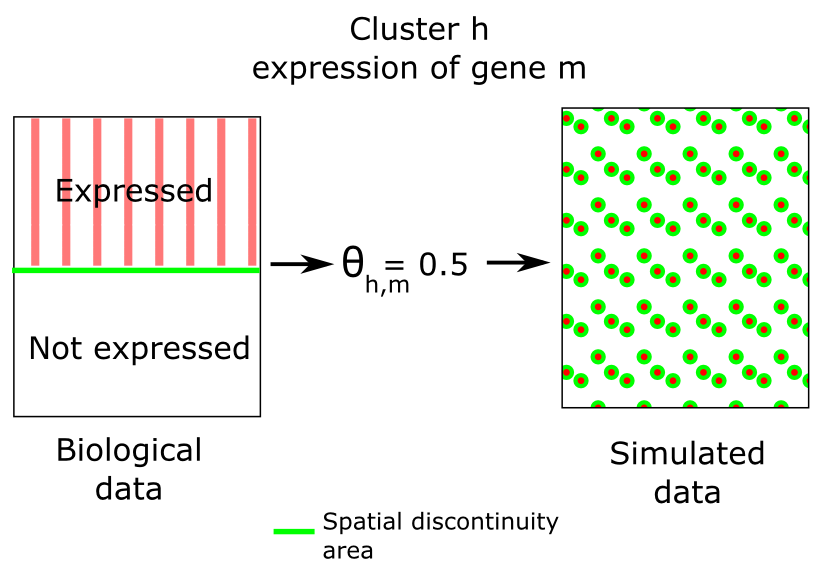
\includegraphics[width=\linewidth]{gfx/chapter5/beta_error.png}}
\caption{{\bf Decrease in spatial coherency due to the simulation scheme.} For an example cluster $h$, gene $m$ may only be expressed in half of the cells. This will yield $\theta_{h,m} = 0.5$. However, in the biological data, the cells expressing gene $m$ may be spatially coherent (i.e., located close to one another), leading to a reduced area of expression discontinuity (the green line). By contrast, in the simulated data the expression of such a gene will lose its spatial coherency, leading to an increased area of expression discontinuity. The number of cells having a neighbour with some differences in the gene expression pattern is directly linked to the value of $\beta_h$ through the energy function (Methods). This explains the underestimation of $\mathbf{\beta}$ observed in Figure \ref{fig:beta_validation}.}
\label{fig:beta_error}
	\end{figure}

To validate further our estimation of $\mathbf{\beta}$, we randomized the coordinates of the ``cubes" to lose any spatial component before re-clustering the data. As expected, we observed that the estimates of $\mathbf{\beta}$ were very close to $0$ for all clusters (Figure \ref{fig:beta_validation}),  as well as there being very similar Jaccard coefficient values (relative to the true values) for the independent mixture and the MRF model. Both of these observations provide confidence in our assertion that the spatial component plays an important role in the fit.\\
	\subsection{Estimation of theta}
	The most important criterion for assessing the efficacy of our approach is the similarity between the inferred and true clusters. This also implicitly assesses the accuracy of the estimation of $\mathbf{\Theta}$: if the inferred and true clusters are identical, the estimates of $\mathbf{\Theta}$ must be equal to the true values. In practice, we used the Jaccard coefficient to compare the inferred and the true clusters (Methods), where a Jaccard coefficient of 1 implies perfect agreement. To benchmark our approach's performance, we also assessed the ability of two other models to cluster the simulated data: hierarchical clustering (hClust), a very widely used approach in genomics and elsewhere, and an independent mixture model, which allows the relative improvement in performance added by the spatial component to be studied.\\
	
		\begin{figure}[h]
\centerline{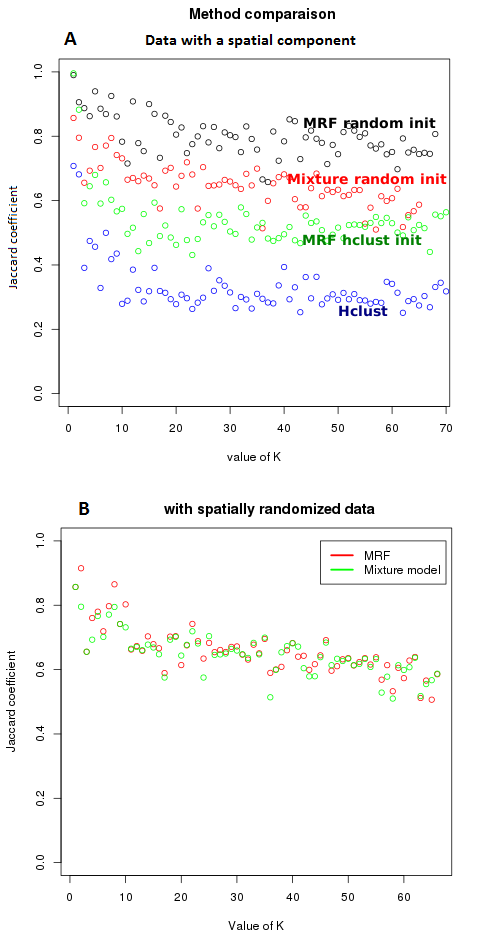
\includegraphics[width=\linewidth]{gfx/chapter5/method_comparison.png}}
\caption{{\bf Jaccard coefficient between ``true" and resulting clusters on the simulated data with different methods and initializations.} Panel A compares the performance of the MRF method with a randomly initialization with an independent mixture model also with a random initialization, the MRF method initialized with the hClust classification and hClust alone on data simulated with a spatial component. Panel B shows the Jaccard coefficient for the MRF method and independent mixture model both with a random initialization; in this case both methods are applied to simulated data that lacks a spatial component.}

\label{fig:methodComparison}
	\end{figure}
	
	The results of these experiments are shown in Figure \ref{fig:methodComparison} for $\tilde{K} \in [4,70]$. Our method, when used with a random initialization scheme (Methods), has an average Jaccard coefficient of $0.8$, and clearly demonstrates better performance than the other methods. The second best performing method is the independent mixture model with a random initialization, which has an average Jaccard coefficient of $0.7$. Since the independent mixture approach is equivalent to the MRF with all the $\beta$ parameters set equal to 0 (i.e., without a spatial component) this suggests that accounting for the spatial aspect yields improved results. Given this, it is perhaps unsurprising that hClust also performs relatively poorly. Additionally, we note that initializing the MRF with the hClust output yields results that are superior to those generated by hClust but that are still poorer than either the randomly initialized independent mixture model or the MRF approach. This is likely explained by noting that, depending upon the initialization, the EM algorithm might converge to a local maximum. Consequently, for the rest of this study we use the random initialization strategy to initialize the EM algorithm. \\
	\subsection{Choosing K}
	
Finally, we assessed the ability of the model to choose the correct number of clusters, $K$. To do this, we noted the ``true" number of clusters underlying the simulated data and compared this with the chosen value, $\hat{K}$. The results for two representative choices of $K$ are shown in Figure \ref{fig:simulatedK} and demonstrate that our clustering approach, in conjunction with the BIC, is able to accurately determine the optimal number of clusters.\\

	\begin{figure}[h]
\centerline{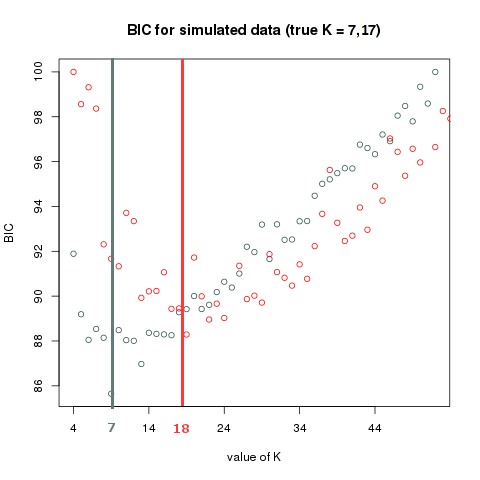
\includegraphics[width=\linewidth]{gfx/chapter5/simulated_k.png}}
\caption{{\bf Jaccard coefficient between ``true" and resulting clusters on the simulated data with different methods and initializations.} Panel A compares the performance of the MRF method with a randomly initialization with an independent mixture model also with a random initialization, the MRF method initialized with the hClust classification and hClust alone on data simulated with a spatial component. Panel B shows the Jaccard coefficient for the MRF method and independent mixture model both with a random initialization; in this case both methods are applied to simulated data that lacks a spatial component.}

\label{fig:simulatedK}
	\end{figure}

\section{Method performance and initialization}
	\subsection{Shortcomings of the EM principle}
	\subsection{Random initialization vs Hclust initialization}
	Additionally, the likelihood function that needs to be maximised possesses many stationary points of different natures. Thus, convergence to the global maximum with the Expectation-maximisation algorithm (see Methods section), depends strongly on the parameter initialisation. To overcome this problem, different initialisation strategies have been proposed and investigated (see for instance \cite{biernacki03,karlis03,mclachlan04}). Herein, we compare a random initialisation scheme with an initialisation based upon the solution obtained by applying hClust.\\

\section{Method performance compared to Hclust and independent mixture models}
	\subsection{Results of comparison}
	\subsection{Discussion}





%*****************************************
%*****************************************
%*****************************************
%*****************************************
%*****************************************
